
\subsection*{1.}

Il y a \(100 - 80 = 20\,\%\) de boules de neige, et parmi celles-ci, \(100 - 32 = 68\,\%\) mesurent moins de 1{,}10 m.

Il y a donc : \(\dfrac{20}{100} \times \dfrac{68}{100} = \dfrac{1360}{10000} = \dfrac{13,6}{100}, \text{ soit }13{,}6\,\% \text{ et donc moins de } 15\,\%\).

\subsection*{2.}

\(p_L(\overline{T})\) désigne la probabilité de l'événement : « sachant que le \(\textit{viburnum}\) choisi est un laurier tin, quelle est la probabilité qu'il mesure moins de 1{,}10 m ? ».

L'événement \(\overline{L} \cap T\) correspond à : « le \(\textit{viburnum}\) choisi est un boule de neige mesurant plus de 1{,}10 m ».

\subsection*{3.}

\begin{center}
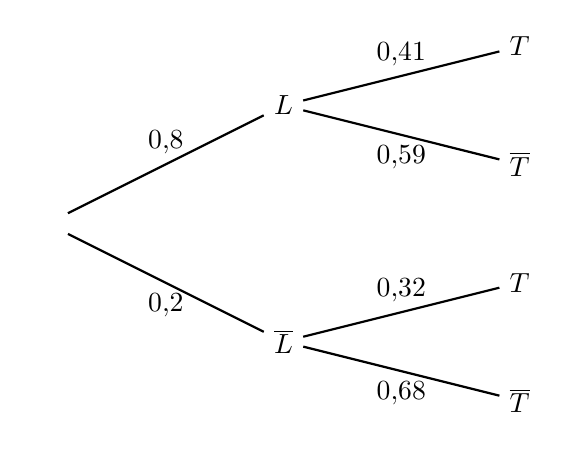
\begin{tikzpicture}[thick, scale=1.5]
\node (P_-1_0) at (-2,-1.5) {$\phantom{A}$};
\node (P_0_0) at (0,-0.5) {$L$};
\draw (P_-1_0) -- (P_0_0) node[midway, above] {$0{,}8$};
\node (P_1_0) at (2,-0) {$T$};
\draw (P_0_0) -- (P_1_0) node[midway, above] {$0{,}41$};
\node (P_1_1) at (2,-1) {$\overline{T}$};
\draw (P_0_0) -- (P_1_1) node[midway, below] {$0{,}59$};
\node (P_0_2) at (0,-2.5) {$\overline{L}$};
\draw (P_-1_0) -- (P_0_2) node[midway, below] {$0{,}2$};
\node (P_1_2) at (2,-2) {$T$};
\draw (P_0_2) -- (P_1_2) node[midway, above] {$0{,}32$};
\node (P_1_3) at (2,-3) {$\overline{T}$};
\draw (P_0_2) -- (P_1_3) node[midway, below] {$0{,}68$};
\end{tikzpicture}
\end{center}

\subsection*{4.}

On a : \(p(T) = p(L \cap T) + p(\overline{L} \cap T)\),

soit : \(p(L \cap T) = p(L) \times p_L(T) = 0{,}8 \times 0{,}41 = 0{,}328\),

et : \(p(\overline{L} \cap T) = p(\overline{L}) \times p_{\overline{L}}(T) = 0{,}2 \times 0{,}32 = 0{,}064\),

Donc : \(p(T) = 0{,}328 + 0{,}064 = 0{,}392\).

\subsection*{5.}

Il faut trouver :
\[
p_{\overline{T}}({\overline{L}}) = \dfrac{p({\overline{T}} \cap {\overline{L}})}{p({\overline{T}})} = \dfrac{0{,}2 \times 0{,}68}{1 - 0{,}392} = \dfrac{0{,}136}{0{,}608} \approx 0{,}2236,
\]
soit \(0{,}224\) au millième près.

